

%\documentclass[pageno]{jpaper}

%replace XXX with the submission number you are given from the ASPLOS submission site.
%\newcommand{\asplossubmissionnumber}{968}

%\usepackage[normalem]{ulem}
%
\newcommand{\mycaption}[3]{\beforecaption\caption{\label{#1}{\bf #2} \em\small #3}\aftercaption}

\newcommand{\BigO}[1]{${\cal O}(#1)$}
\newcommand{\BigOmega}[1]{$\Omega(#1)$}
\newcommand{\BigTheta}[1]{$\Theta(#1)$}

% only foreign words should be italicized... (example given should not)
\newcommand{\eg}{\textit{e.g.}}
\newcommand{\ie}{\textit{i.e.}}
\newcommand{\etal}{\textit{et al.}}
\newcommand{\etc}{\textit{etc.}}
\newcommand{\adhoc}{\textit{ad hoc}}

% units
\newcommand{\KB}{\,KB}
\newcommand{\MB}{\,MB}
\newcommand{\GB}{\,GB}
\newcommand{\TB}{\,TB}
\newcommand{\MBs}{\,MB/s}
\newcommand{\KBs}{\,KB/s}
\newcommand{\Kbs}{\,Kbit/s}
\newcommand{\mbs}{\,Mbit/s}
\newcommand{\mus}{\mbox{\,$\mu s$}}
\newcommand{\ms}{\mbox{\,$ms$}}

\renewcommand{\em}{\it}
\newcommand{\x}{$\times$}

% lego
\newcommand{\splitkernel}{splitkernel}
\newcommand{\lego}{LegoOS}
\newcommand{\ib}{IB}
\newcommand{\ibverbs}{IB-Verbs}
\newcommand{\rdma}{RDMA}
\newcommand{\dcrack}{DC-Rack}
\newcommand{\vnode}{vNode}
\newcommand{\vip}{vIP}
\newcommand{\vmount}{vMount}
\newcommand{\mmap}{{\texttt{mmap}}}
\newcommand{\munmap}{{\texttt{munmap}}}
\newcommand{\mremap}{{\texttt{mremap}}}
\newcommand{\grm}{GRM}
\newcommand{\gmm}{GMM}
\newcommand{\gsm}{GSM}
\newcommand{\gpm}{GPM}
\newcommand{\excache}{ExCache}
\newcommand{\vicache}{VtmCache}
\newcommand{\vregion}{vRegion}
\newcommand{\microos}{monitor}
%\newcommand{\microos}{$\mu$OS}
\newcommand{\brk}{{\texttt{brk}}}
\newcommand{\pcomponent}{pComponent}
\newcommand{\mcomponent}{mComponent}
\newcommand{\scomponent}{sComponent}

% dsnvm
\newcommand{\dsnvm}{DSPM}
\newcommand{\dsm}{DSM}
\newcommand{\nvm}{PM}
\newcommand{\hotpot}{Hotpot}
\newcommand{\mrmw}{MRMW}
\newcommand{\mrsw}{MRSW}
\newcommand{\wfetch}{FETCH}
\newcommand{\cd}{CD}
\newcommand{\dr}{DR}
\newcommand{\on}{ON}
\newcommand{\dn}{DN}
\newcommand{\xn}{CN}
\newcommand{\master}{MN}
\newcommand{\xactid}{CID}
\newcommand{\dirty}{dirty}
\newcommand{\committed}{committed}
\newcommand{\redundant}{redundant}
\newcommand{\ib}{IB}
\newcommand{\sendreply}{\texttt{send-reply}}
\newcommand{\atomicsendreply}{\texttt{atomic-send-reply}}
\newcommand{\multisendreply}{\texttt{multicast-send-reply}}
\newcommand{\journaled}{JOURNALED}
\newcommand{\fsyncsafe}{FSYNC\_SAFE}
\newcommand{\X}{{$\times$}}
\newcommand{\pmfs}{PMFS}
\newcommand{\tmpfs}{tmpfs}
\newcommand{\Octopus}{Octopus}
\newcommand{\Mojim}{Mojim}
\newcommand{\dsmnoxact}{DSM-NoXact}
\newcommand{\dsmxact}{DSM-Xact}
\newcommand{\clflush}{\texttt{clflush}}
\newcommand{\pcommit}{\texttt{pcommit}}
\newcommand{\mfence}{\texttt{mfence}}
\newcommand{\sfence}{\texttt{sfence}}
\newcommand{\ra}{\textbf{R1.a}}
\newcommand{\rb}{\textbf{R1.b}}
\newcommand{\rcs}{\textbf{R2.a}}
\newcommand{\rcm}{\textbf{R2.b}}
\newcommand{\rdr}{\textbf{R3.r}}
\newcommand{\rdu}{\textbf{R3.u}}
\newcommand{\re}{\textbf{R3}}
\newcommand{\rf}{\textbf{R4}}

%
\newcommand{\mm}{mm$^2$}
\newcommand{\figtitle}[1]{\textbf{#1}}
\newcommand{\us}{$\mu$s}
\newcommand{\fixme}[1]{{\color{red}\textbf{#1}}}

\definecolor{pink}{rgb}{1.0,0.47,0.6}
\newcommand{\adrian}[1]{{\color{green}\textbf{#1}}}
\newcommand{\laura}[1]{{\color{pink}\textbf{#1}}}
\newcommand{\joel}[1]{{\color{red}\textbf{#1}}}
\newcommand{\ameen}[1]{{\color{blue}\textbf{#1}}}
\newcommand{\arup}[1]{{\color{yellow}\textbf{#1}}}
\newcommand{\hungwei}[1]{{\color{purple}\textbf{#1}}}


\newcommand{\note}[2]{\fixme{$\ll$ #1 $\gg$ #2}}

\newcommand{\myitem}[1]{\item \textbf{#1}}

\lstloadlanguages{% Check Dokumentation for further languages ...
        %[Visual]Basic
        %Pascal
        C
        %C++
        %XML
        %HTML
        %Java
}

\lstdefinestyle{customc}{
  belowcaptionskip=1\baselineskip,
  breaklines=true,
  frame=b,
  xleftmargin=\parindent,
  language=C,
  showstringspaces=false,
  basicstyle=\scriptsize\ttfamily,
  keywordstyle=\bfseries\color{green!40!black},
  commentstyle=\itshape\color{purple!40!black},
  identifierstyle=\color{blue},
  stringstyle=\color{red},
}
\lstset{escapechar=@,style=customc}

%\usepackage[numbers,sort]{natbib}

%\begin{document}

\title{Clio: A Hardware-Software Co-Designed Disaggregated Memory System \\ \textbf{Extended Abstract}\vspace{-0.3in}}

\date{}

\maketitle

\thispagestyle{empty}

%\section{Introduction and Motivation}
%\label{sec:intro}






\section{Motivation}

Modern data-center applications like graph computing, data analytics, and deep learning have increasing demand for access to large amounts of memory~\cite{FastSwap}.
Unfortunately, servers are facing {\em memory capacity walls} because of pin, space, and power limitations~\cite{HP-MemoryEvol,ITRS14,MemoryWall95}.
Going forward, it is imperative for datacenters to seek solutions that can go beyond what a (local) machine can offer, \ie, using remote memory.
At the same time, data centers are seeing the needs from management and resource utilization perspectives
to {\em disaggregate} resources~\cite{Ali-SinglesDay,SnowFlake-NSDI20,FB1}\textemdash separating hardware resources into different network-attached pools 
that can be scaled and managed independently.
These real needs have pushed the idea of memory disaggregation ({\em \md} for short):
organizing computation and memory resources as two separate network-attached
pools, one with compute nodes ({\em CN}s) and one with memory nodes ({\em MN}s).

\section{Limitations of the State of the Art}
So far, \md\ research has all taken one of two approaches,
building/emulating \MN{}s with either regular servers~\cite{AIFM,InfiniSwap,FastSwap,Shan18-OSDI,zombieland} 
or raw memory devices with no processing power~\cite{Tsai20-ATC,Lim09-disaggregate,Lim12-HPCA,HP-TheMachine}.
%,ATC21Paper
%\textit{Is it possible to build \MN{}s without a server}, as promised by the original proposal of \md~\cite{Lim09-disaggregate,Shan18-OSDI}?
The fundamental issues of server-based approaches such as RDMA-based systems are the monetary cost of a host server and the inherent performance and scalability limitations caused by the way NICs interact with the host server's virtual memory system.
Raw-device-based solutions have low costs.
However, they introduce performance, security, and management problems
because when \MN{}s have no processing power, all the data and control planes have to be handled at \CN{}s~\cite{Tsai20-ATC}.
%\MN{}s become too ``dumb'' and low level when removing its processing power altogether.
%overhead of root cause why RDMA is unfit for \md\ is that it is designed to work around a host server,
%and traditional servers' virtual memory system is not designed for \md.
%Contrary to server-based \md\ solutions, \pdm\ is another extreme where there is no processing at all at \MN{}s.
%The root cause of \pdm's various performance, security, and management problems is exactly this: 
%\MN{}s are too ``dumb'' and low level.

%From the above discussion, we find that both server-based \md\ and raw physical \md\ have their limitations.
Server-based \MN{}s and \MN{}s with no processing power are two extreme approaches of building \MN{}s.
We seek a sweet spot in the middle by proposing a hardware-based \md\ solution that has the right amount of processing power at \MN{}s.
%for the right type of \MN{} management system.
%To mitigate RDMA's various issues for \md, one could try to improve RDMA's hardware design or add a software layer to work around RDMA's problems.
%This paper takes a different approach by starting
Furthermore, we take a clean-slate approach by starting from the requirements of \md\
and designing a \md-native system.
%LegoOS is the only existing work that also proposes a .
%Unfortunately, LegoOS still uses server software and the RDMA network to emulate its hardware design, leaving all the research questions we ask in this paper unanswered.

\section{Key Insights and Proposal}

{
\begin{figure*}[th]
\begin{subfigure}{1.7in}
\begin{center}
\centerline{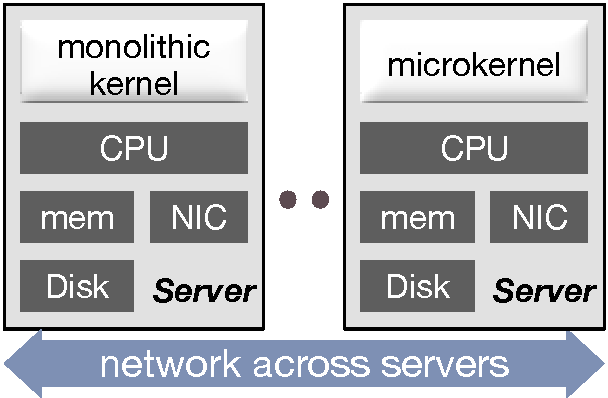
\includegraphics[width=1.7in]{lego/Figures/monolithic-arch.pdf}}
\caption[Monolithic OS.]{OSes Designed for Monolithic Servers.}
\label{fig-monolithic}
\end{center}
\end{subfigure}
\begin{minipage}{0.05in}
\hspace{0.05in}
\end{minipage}
\begin{subfigure}{1.8in}
\begin{center}
\centerline{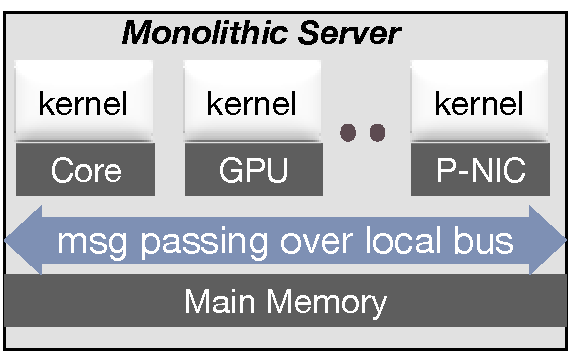
\includegraphics[width=1.8in]{lego/Figures/multikernel-arch.pdf}}
\caption[Multikernel Architecture.]{Multi-kernel Architecture. \small{P-NIC: programmable NIC.}}
\label{fig-multikernel}
\end{center}
\end{subfigure}
\begin{minipage}{0.05in}
\hspace{0.05in}
\end{minipage}
\begin{subfigure}{2.5in}
\begin{center}
\centerline{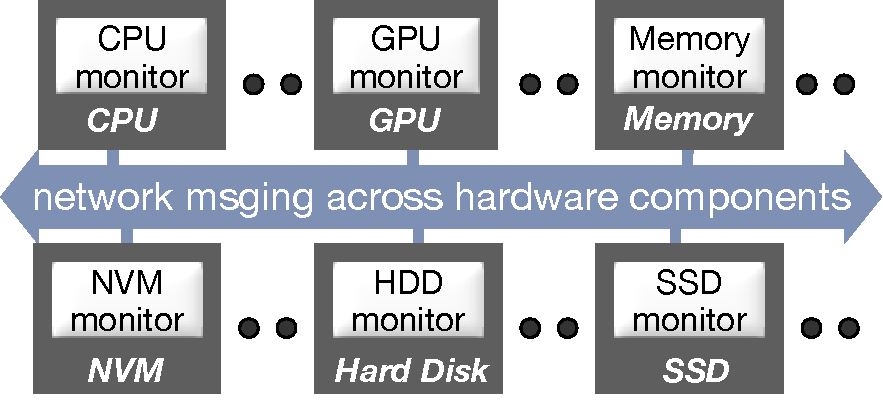
\includegraphics[width=2.6in]{lego/Figures/lego-arch.pdf}}
\caption[Splitkernel Architecture.]{Splitkernel Architecture.}
\label{fig-splitkernel}
\end{center}
\end{subfigure}
\caption[Operating System Architecture.]{Operating System Architecture.}
\end{figure*}
}

We built {\em \sys}, a hardware-based disaggregated memory system (Figure~\ref{fig-arch}).
%focusing on the hardware-based virtual memory system and network stack.
\sys\ includes a \CN-side user-space library called {\em \syslib}
and a new hardware-based \MN\ device called {\em \sysboard}.
Multiple application processes running on different \CN{}s could allocate memory from the same \sysboard, with each process having its own {\em remote virtual memory address space}.
Applications access their remote memory space using APIs that \sys\ provides (\eg, \alloc, \sysread, \syswrite, \syslock), and the accesses are in byte granularity.
For each API, \sys\ provides a synchronous version and an asynchronous version, with the former following sequential consistency and the latter following release consistency.

A \sysboard\ consists of three main components: 1) a hardware chip that integrates a thin network stack and a virtual memory system to handle data requests (the {\em fast path}), 2) an ARM processor that runs software to handle metadata requests and background tasks (the {\em slow path}), and 3) an FPGA that hosts application computation offloading (the {\em extend path}).

In building \sys, we explore new requirements, challenges, and benefits of \md.
Specifically, we answer three important research questions.

First, \textbf{how does the design and implementation of a
dedicated hardware \MN\ differ from server and programmable NIC
designs?}
%To protect the accesses from different applications to the memory in an \MN\ and to make such accesses flexible, 
%we should use a virtual memory system to check and map virtual memory addresses to physical addresses.
Current \md\ solutions rely on a host server (its OS and MMU) to provide a virtual memory system so that accesses to the memory are protected and flexible. 
Using a whole server just for the virtual memory system is overkill and unnecessarily adds monetary and energy costs to \md. %consumes too much power.
Another possibility is to use a low-power processor (\eg, ARM) in a SmartNIC to run the virtual memory system~\cite{iPipe}. 
However, doing so has high performance impact mainly because the virtual memory system is on a separate chip from the NIC.
%However, doing so has performance overhead, both because the virtual memory system is on a separate chip from the NIC
%and because the virtual memory system is not designed for \md.
%To date, there has been no attempt
%\yizhou{I think here we should emphasize that: MNs emulated using host server has cost and power waste while the SmartNIC-based ones have perf issue. In all, there is no ideal solution for building real server-less MNs. Hence we took a ...}
Overall, server-based approaches have cost overheads while SmartNIC solutions have performance overheads.
We took a clean-slate approach by building a hardware-based virtual memory system that is integrated with a customized hardware network stack, 
both of which are designed specifically for handling virtual memory requests sent over the network.

Second, \textbf{how can a low-cost \MN\ host TBs of memory and support thousands of concurrent application processes?}
Different from traditional (local) memory, an \MN\ is intended to be shared by many applications running at different \CN{}s,
and the more applications it can support, the more efficiently its memory can be utilized.
Thus, we aim to have each \MN\ host TBs of memory for thousands of concurrent applications processes.
However, a hardware design is constrained by the limited resources in a hardware chip such as on-chip memory.
Compared to traditional software-based virtual memory systems, 
how can an \MN\ use orders of magnitude less resources while achieving orders of magnitude higher scalability?
%which raises the problem of how to manage the scalability we target in hardware.
%is especially accute in an \hdm\ because of its low cost requirements.
Current solutions like RDMA NICs swap metadata between NIC's on-chip memory and host server memory,
which comes with performance overhead (4\x\ compared with when metadata is in the NIC memory~\cite{Pythia}).
%RDMA improves scalability by adding more hardware resources to cache more metadata/states), which comes with increasing monetary and energy costs.

Our clean-slate approach is to carefully examine each virtual-memory and networking task 
and to redesign them to \textbf{1)} eliminate states and metadata whenever possible (\eg, by eliminating the RDMA "Memory-Region" concept),
\textbf{2)} move complex but non-performance-critical states, metadata, and tasks to the software slow path,
\textbf{3)} shift functionalities to the \CN\ (\syslib) to reduce \MN's complexity 
(\eg, our reliable network transport runs at \syslib, and \MN\ is ``transport-less''; we achieve reliability by ordering and retrying at the memory request level instead of the packet level),
and \textbf{4)} design bounded-size, inherently scalable data structures (we propose a new page table design that lets all processes share one global page table whose size is determined by the physical memory size).
%For the remaining functionalities that still need caching, we redesign them to guarantee good cache-miss performance.
As a result, each \MN\ (\sysboard) could support TBs of memory and thousands of application processes with only 1.5\MB\ on-chip memory.
%\yizhou{On top of network scalability, I think its also worth explaining how we are able to support TBs of memory. Because this reminds me of O(1) memory issues. With TBs of memory, the memory related metadata and OPs increased as well. Our pros: our fast path use huge page + hashtable-based pgtable, bounded latency. Our cons: our buddy allocator running in ARM is still prone to this huge memory issue.}
%For certain functionalities, we avoid states and metadata alltogether by re-designing the functionalities.
%For functionalities that could be and move the ones that can be moved to the \CN\ side.
%and not relying on cache for good performance.

Third, \textbf{how to minimize tail latency in a \md\ system}?
%\textbf{is it possible to minimize tail latency by processing all read/write requests deterministically?} 
Tail latency is important in data centers especially for workloads that have large fanouts (\eg, Spark jobs).
Although much effort has focused on improving the network and core scheduling for low tail latency~\cite{nanoPU,Shenango,Shinjuku,ZygOS,RPCValet},
the memory system has largely been overlooked.
However, the (remote) memory system is what contributes to extreme long tails in a \md\ system.
For example, RDMA's round-trip latency is around 1--2\mus\ in the common case,
but its tail could be as long as 16.8\ms. % (when there is a page fault).
%The main reason for RDMA's various tails is its reliance on the host virtual memory system, which is not designed for \md\ or for low tail latency.

We reexamine traditional memory system
%from the tail latency and perspectives 
and propose a set of novel mechanisms to bound \sys's tail latency.
Our core idea is to include {\em all} the functionalities that are needed to fulfill all types of data requests in one hardware pipeline
and to make this hardware pipeline {\em performance deterministic}.
This pipeline takes one incoming data unit every cycle (\ie, no pipeline stalls) and completes every request in a fixed number of cycles.
Two major technical hurdles in achieving this performance are to perform page table lookups and to handle page faults in a bounded, short time period.  
For the former, we propose a new {\em overflow-free} hash-based page table that bounds all page table lookups to {\em at most one DRAM access} (instead of the long page table walk in a traditional CPU architecture).
Our novel idea is to avoid overflows at the virtual memory address allocation time, by retrying the allocation until a non-overflow virtual memory address range is found.
For the latter, we propose a new mechanism to handle page faults in hardware with bounded cycles (instead of the costly process of interrupting and handling page faults in OS).

%These mechanisms include 1) handling page faults in hardware,
%2) d
%RDMA’s way is to pre-reserve memory and to use large on-device cache. But cache can’t always work, and reserving memory results in inefficient memory utilization.
%Our solution is to allocate physical memory on-demand and to make the cache miss path fast by handling page faults in hardware and by designing a new hash-based page table. We also carefully designed our hardware pipeline to have deterministic, bounded latency.

\section{Main Artifacts and Key Results}

{
\begin{figure*}[th]
\begin{center}
\centerline{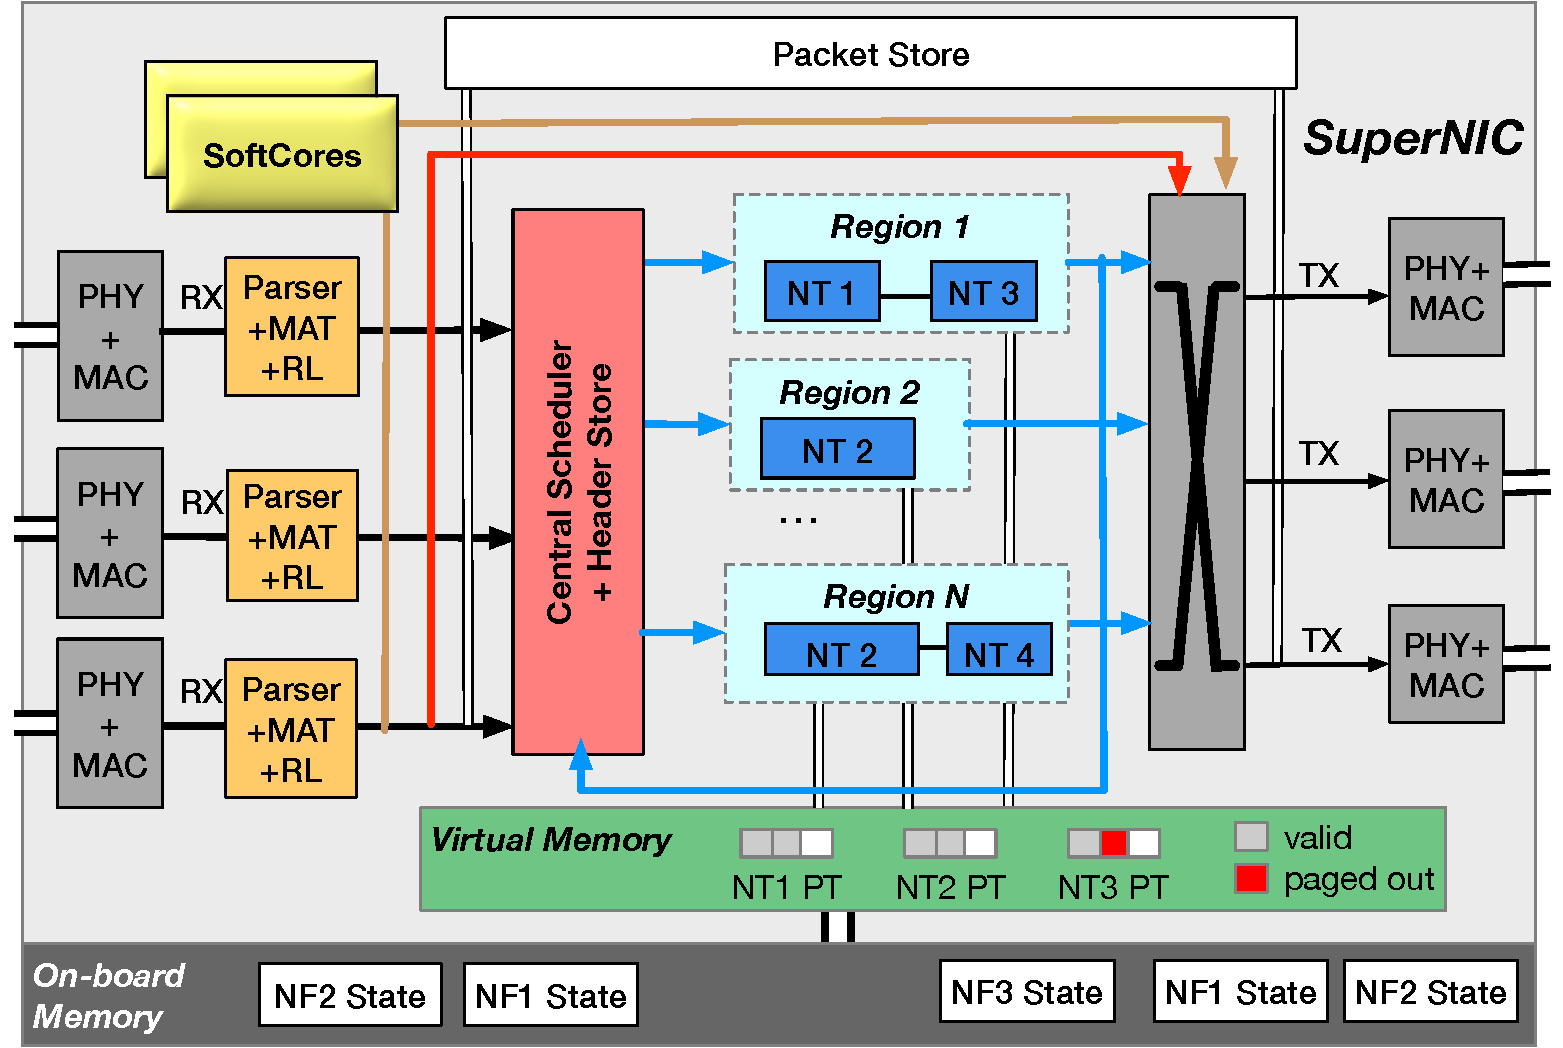
\includegraphics[width=\textwidth]{snic/Figures/board.pdf}}
\mycaption{fig-snic-board}{\snic\ On-Board Design.}
{
RL: Rate Limiter. PT: Page Table
}
\end{center}
\end{figure*}
}
{
\begin{figure*}[th]
\begin{center}
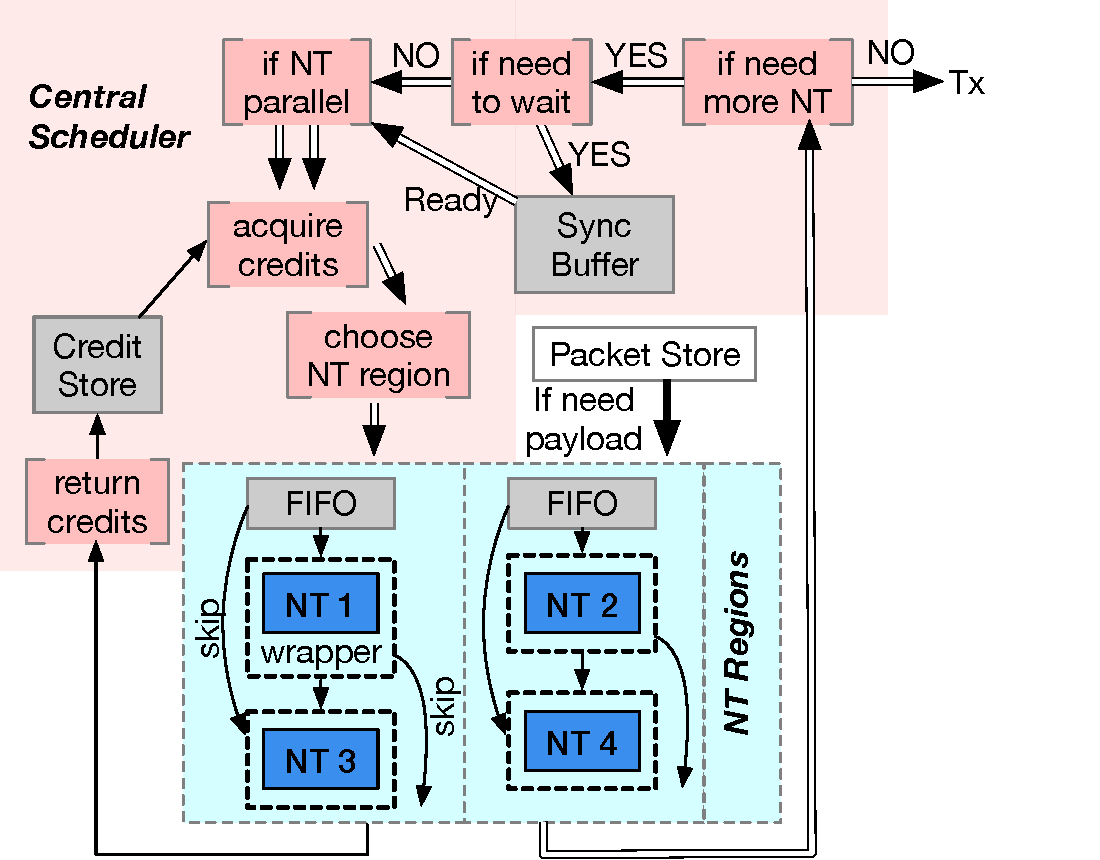
\includegraphics[width=0.9\textwidth]{snic/Figures/scheduler.pdf}
\mycaption{fig-sched}{\snic\ Packet Scheduler and \nt\ Region Design.}
{
Double arrows, single arrows, and thick arrows represent packet headers, credits, and packet payload.
}
\end{center}
\end{figure*}
}

We prototyped \sysboard\ with a Xilinx MPSoC FPGA board~\cite{ZCU106} and implemented \syslib\ as a user-space library on Linux servers. 
Figure~\ref{fig-coremem} illustrates the overall board-level design.
We built three applications using \sys:
a FaaS-style image compression utility, a radix-tree index, and a key-value store.
%We prototyped \sys's memory device with FPGA (\sysboard).
%\sys\ achieves high throughput (100\Gbps\ with FPGA prototype), low (tail) latency (XXX\mus\ end-to-end MTU round trip latency), 
%low cost (XXX\x\ energy saving), %and great extendibility,
%and \sys\ scales well with XXX. %eliminates {\em all} scalability bottlenecks in both its memory and network systems.
Our FPGA \sys\ prototype achieves 100\Gbps\ throughput and an end-to-end latency of 2.5\mus\ at median and 3.2\mus\ at 99-percentile.
We compared \sys\ with native RDMA, two RDMA-based disaggregated/remote memory systems~\cite{Tsai20-ATC,Kalia14-RDMAKV}, 
a software emulation of hardware-based disaggregated memory LegoOS~\cite{Shan18-OSDI},
%an FPGA-based RDMA implementation~\cite{StRoM}, 
and a software-based SmartNIC BlueField~\cite{BlueField}.
\sys\ scales much better and has orders of magnitude lower tail latency than RDMA, 
while achieving similar throughput and median latency as RDMA (even with the slower FPGA frequency in our prototype).
\sys\ has 1.1\x\ to 3.4\x\ energy saving compared to CPU-based and SmartNIC-based disaggregated memory systems 
and is 2.7\x\ faster than software-based SmartNIC solutions. 
%We will make \sys\ publicly available upon this paper's publication.


Overall, this paper makes the following contributions.

\begin{itemize}

\item The first publicly described hardware-based disaggregated memory system and an FPGA prototype.

\item A demonstration of how to co-design system software (a full virtual memory system), hardware architecture (memory management unit), and networking stack (a customized reliable network).

\item A demonstration of how to co-design the compute and the memory sides in a disaggregated system.

\item A demonstration of how to separate data and control plane in a virtual memory system for disaggregated memory.

\item Three applications built with real disaggregated memory, with some offloading their computation to memory devices.
%\item Hardware-based distributed operation support such as migration and replication.

% and a set of extended virtual memory APIs. 
%\item Demonstration of how real systems could use and benefit from disaggregated memory services.

%\item Two hardware-based high-level distributed memory services.
%\item Demonstration of two deployment models of disaggregated memory hardware.

\end{itemize}



%\subsection*{Why ASPLOS}
%\label{sec:why-asplos}
\section{Why ASPLOS}
This paper demonstrates how to implement a core OS functionality, the virtual memory system, in hardware in a non-conventional way.
We also demonstrate how to co-design hardware and software.
Thus, this paper fits well with the scope of ASPLOS in
architecture and system.
 
\pagebreak
%\bibliographystyle{plain}
%\bibliography{all-defs,all,personal,all-confs,local,paper}


%\end{document}

